\documentclass[12pt]{ruthesis}

\pdfinterwordspaceon
\pdfminorversion=8

\widowpenalty10000
\clubpenalty10000
\interfootnotelinepenalty=200

\RequirePackage{amsmath}

\RequirePackage[hang,flushmargin]{footmisc}
\RequirePackage{setspace}

\RequirePackage{caption}

\RequirePackage[usenames,dvipsnames,svgnames,table]{xcolor}
\RequirePackage{microtype}
% Disables fi -> fi type ligatures
\DisableLigatures[f]{}

\RequirePackage{dcolumn}
\RequirePackage{longtable}
\RequirePackage{tabularx}
\RequirePackage{afterpage}

\usepackage[pdftex,
            pdfpagelayout = OneColumn,
            pdfpagemode = UseOutlines,
            %TODO: Change these two values.
%            pdftitle = "Risk Fact or Fiction: The Information Content of Risk Factor Disclosures",
            pdftitle = {Risk Fact or Fiction: The Information Content of Risk Factor Disclosures},
            pdfauthor = {Maclean Gaulin},
            pdfdisplaydoctitle = true,
            bookmarks,
            bookmarksopen = true,
            bookmarksnumbered = false,
            breaklinks = true,
            hidelinks,
            colorlinks = false,
            hyperindex = true,
            hyperfigures]{hyperref}
	\newcommand{\bluehref}[2]{{\color{blue}\href{#1}{#2}}}


\RequirePackage[comma,longnamesfirst]{natbib}
\RequirePackage{booktabs}

%%%%%%%%%%%%%%%%%%%%%%%%%%%%%%%%%%%%%%%%%%%%%%%%%%%%%%%%%%%%%%%%%%%%%%%%%%%%%%%%%%%%%%%%%%%%%%
%   .d8888b.                    888                          d8b                             %
%  d88P  Y88b                   888                          Y8P                             %
%  888    888                   888                                                          %
%  888        888  888 .d8888b  888888 .d88b.  88888b.d88b.  888 88888888  .d88b.            %
%  888        888  888 88K      888   d88""88b 888 "888 "88b 888    d88P  d8P  Y8b           %
%  888    888 888  888 "Y8888b. 888   888  888 888  888  888 888   d88P   88888888           %
%  Y88b  d88P Y88b 888      X88 Y88b. Y88..88P 888  888  888 888  d88P    Y8b.               %
%   "Y8888P"   "Y88888  88888P'  "Y888 "Y88P"  888  888  888 888 88888888  "Y8888            %
%                                                                                            %
%                 The following variables to reflect your thesis.                            %
%%%%%%%%%%%%%%%%%%%%%%%%%%%%%%%%%%%%%%%%%%%%%%%%%%%%%%%%%%%%%%%%%%%%%%%%%%%%%%%%%%%%%%%%%%%%%%

\ctitle{Risk Fact or Fiction:\\The Information Content of\\Risk Factor Disclosures}
\title{Risk Fact or Fiction: The Information Content of Risk Factor Disclosures}
\author{Maclean Gaulin}
\department{Accounting, Jones Graduate School of Business}
\school{Rice University}
\degree{Doctor of Philosophy}

% Change this to Rice shield and name, or your department's name.
\coverart{
\includegraphics{RiceBusiness_JGSB_2c_VectorShield.eps}}

\committee {
	K. Ramesh, Chair \\
	Herbert S. Autrey Professor of Accounting \and
	Brian Akins \\
	Assistant Professor of Accounting \and
	Brian Rountree \\
	Associate Professor of Accounting \and
	Robin Sickles \\
	Reginald Henry Hargrove Chair of Economics \and
	Shiva Sivaramakrishnan \\
	Henry Gardiner Symonds Professor of Accounting
}

\address{Houston, Texas}
\donemonth{March} \doneyear{2017} \makeindex



%%%%%%%%%%%%%%%%%%%%%%%%%%%%%%%%%%%%%%%%%%%%%%%%%%%%%%%%%%%%%%%%%%%%%%%%%%%%%%%%%%%%%%%%%%%%%%
%   .d8888b.                    888              .d8888b.                     888            %
%  d88P  Y88b                   888             d88P  Y88b                    888            %
%  888    888                   888             888    888                    888            %
%  888        888  888 .d8888b  888888          888        88888b.d88b.   .d88888 .d8888b    %
%  888        888  888 88K      888             888        888 "888 "88b d88" 888 88K        %
%  888    888 888  888 "Y8888b. 888             888    888 888  888  888 888  888 "Y8888b.   %
%  Y88b  d88P Y88b 888      X88 Y88b.  d8b      Y88b  d88P 888  888  888 Y88b 888      X88   %
%   "Y8888P"   "Y88888  88888P'  "Y888 Y8P       "Y8888P"  888  888  888  "Y88888  88888P'   %
%%%%%%%%%%%%%%%%%%%%%%%%%%%%%%%%%%%%%%%%%%%%%%%%%%%%%%%%%%%%%%%%%%%%%%%%%%%%%%%%%%%%%%%%%%%%%%
\newcommand{\skipline}{\vspace{12pt}}
\newcommand{\tablesize}{\scriptsize}


\newenvironment{thesistable}[2]%
{ % Begin begin
    \newcommand{\postamble}{The variables are defined in Appendix \ref{App:vardef}.
        Robust standard errors are clustered at the firm level and absolute t-statistics are reported in parentheses.
        ***, **, and * indicate significance at the 0.01, 0.05, and 0.10 level, respectively.}
    \newcommand{\startdata}{\centering \vspace{12pt} \tablesize}

    \bgroup
    % \def\arraystretch{1.2}
    % \setlength\tabcolsep{.1em}
    \begin{table}[!htb]
            \caption{#1}
            \footnotesize
} % End begin
{ % Begin end
    \end{table}
    \egroup
} % End end
\def\sym#1{\ifmmode^{#1}\else\(^{#1}\)\fi}







%%%%%%%%%%%%%%%%%%%%%%%%%%%%%%%%%%%%%%%%%%%%%%%%%%%%%%%%%%%%%%%%%%%%%%%%%%%%%%%%%%%%%%%%%%%%%%
%  888888b.                 888                                                              %
%  888  "88b                888                                                              %
%  888  .88P                888                                                              %
%  8888888K.   .d88b.   .d88888 888  888                                                     %
%  888  "Y88b d88""88b d88" 888 888  888                                                     %
%  888    888 888  888 888  888 888  888                                                     %
%  888   d88P Y88..88P Y88b 888 Y88b 888                                                     %
%  8888888P"   "Y88P"   "Y88888  "Y88888                                                     %
%                                    888                                                     %
%                               Y8b d88P                                                     %
%                                "Y88P"                                                      %
%%%%%%%%%%%%%%%%%%%%%%%%%%%%%%%%%%%%%%%%%%%%%%%%%%%%%%%%%%%%%%%%%%%%%%%%%%%%%%%%%%%%%%%%%%%%%%
\renewcommand{\floatpagefraction}{1}
\begin{document}

\begin{frontmatter}
    \pagenumbering{roman}
    % Comment out to remove flashy cover
    \makecover
    % The maketitle makes the signature page
    \maketitle
    \thispagestyle{empty}
\begin{abstract}

Paper Abstract

\end{abstract}

    \begin{acknowledge}

I am honored to have completed my PhD dissertation under the mentoring and tutelage of Dr. K. Ramesh.

\end{acknowledge}
    \tableofcontents
    \listoffigures
    \listoftables
\end{frontmatter}

\pagenumbering{arabic}

\linespacing{1.7}


%%%%%%%%%%%%%%%%%%%%%%%%%%%%%%%%%%%%%%%%%%%%%%%%%%%%%%%%%%%%%%%%%%%%%%%%
%                            Chapters                                  %
%%%%%%%%%%%%%%%%%%%%%%%%%%%%%%%%%%%%%%%%%%%%%%%%%%%%%%%%%%%%%%%%%%%%%%%%

\chapter{Introduction} \label{ch:introduction}
    
Do managers disclose \textit{risk factors} consistent with the regulatory requirement to warn of \textit{future adverse outcomes}?
Yes.


\chapter{Risk Factor Disclosure Information Content} \label{ch:supply}
    This dissertation studies the information content of mandatory risk factor disclosures filed in annual reports by public firms in the United States.




\section{Hypothesis Development}\label{sec:supply_hypothesis}

The requirement to disclose risk factors is set forth in Item 503(c) of Regulation S-K:
\begin{quote}\singlespacing
	\textbf{\S 229.503 (Item 503) (c) Risk factors}. 
	Where appropriate, provide under the caption ``Risk Factors'' a discussion of the most significant factors that make the offering speculative or risky. 
	This discussion must be concise and organized logically. 
	Do not present risks that could apply to any issuer or any offering. 
	Explain how the risk affects the issuer or the securities being offered. 
	Set forth each risk factor under a subcaption that adequately describes the risk.
\end{quote}



\section{Sample Construction and Data Collection}\label{sec:sample}

Risk Factor disclosures have been required in annual and quarterly disclosures under Item 1A since the SEC regulation took effect in 2005.


\begin{thesistable}{Summary Stats}{\ref{tab:summarystats}}
	\label{tab:summarystats}
	
	Table \ref{tab:summarystats} reports the summary statistics for the variables used in the regressions as defined in Appendix \ref{App:vardef}.
	
	\startdata
	\begin{tabular}{l*{1}{cccccccc}} \toprule
	                                   &  Mean   & Std. Dev &  Min  & 25\%  & 50\%  &  75\%  &  Max   &   N    \\ \midrule
	$ Log(Assets)_{t} $                &  6.70   &   2.01   & 2.12  & 5.34  & 6.74  &  8.05  & 11.56  & 26,547 \\
	$ Log(Market\ Equity)_{t} $        &  6.33   &   1.96   & 1.84  & 4.99  & 6.35  &  7.70  & 10.56  & 26,537 \\
	$ Book-to-Market_{t} $             &  0.73   &   0.90   & -0.71 & 0.31  & 0.58  &  0.96  &  4.60  & 26,518 \\
	$ Sales / AT_{t} $                 &  0.90   &   0.85   & 0.00  & 0.26  & 0.70  &  1.27  &  4.04  & 26,536 \\
	$ Beta_{t-1} $                     &  1.04   &   0.54   & -0.10 & 0.69  & 1.05  &  1.40  &  2.31  & 26,547 \\ \midrule \addlinespace 
    \multicolumn{9}{c}{\normalsize Indicator and Negative Outome Variables}                                    \\ \midrule
	$ Negative\ NI_{t+1} $             &  0.31   &   0.46   &   0   &   0   &   0   &   1    &   1    & 22,026 \\
	$ Sec.\ Litigation_{t-1} $         &  0.02   &   0.14   &   0   &   0   &   0   &   0    &   1    & 26,546 \\
	$ Lawsuit\ Intensity_{t-1} $       &  0.19   &   0.44   &   0   &   0   &   0   &   0    &  2.08  & 26,547 \\
	$ RF\ Comment_{t-1} $              &  0.07   &   0.25   &   0   &   0   &   0   &   0    &   1    & 26,224 \\
	$ Comment\ (Any)_{t-1} $           &  0.53   &   0.50   &   0   &   0   &   1   &   1    &   1    & 26,223 \\ \midrule \addlinespace
    \multicolumn{9}{c}{\normalsize Textual Variables}                                                          \\ \midrule
	$ \#\ Risk\ Factors_{t} $          &  29.52  &  14.05   &   6   &  19   &  27   &   37   &   69   & 26,547 \\
	$ \#\ New\ RF_{t} $                &  3.67   &   5.03   &   0   &   1   &   2   &   5    &   25   & 26,547 \\
	$ \#\ Dropped\ RF_{t} $            &  2.45   &   3.73   &   0   &   0   &   1   &   3    &   21   & 26,547 \\
    $ \Delta \#\ RF_{t} $              &   1.22  &   4.56   & -11   &   0   &   1   &   2    &   18   & 26,547 \\ \bottomrule
\end{tabular}
\end{thesistable}

The average firm in my sample has 29.5 risk factors, and adds 3.7 new risks and removes 2.5 obsolete risks per year.
I find that younger firms (below the median firm age of 13 years) disclose 34.4 risk factors on average, and identify 4.4 new factors per year and remove 3.2 factors.
Older firms (above median age) disclose significantly fewer risk factors, only 25.8, and identify new factors and remove old factors at significantly lower rates as well (3.4 and 2.2, respectively).
This potentially suggests life cycle effects in risk factor disclosures, with older, more established, and less volatile firms disclosing fewer risks and experiencing less risk `turnover.'
However, when looking at the change in word count of the risk factors between these two groups, there is no significant difference.%
\footnote{The change in word counts are 135.5 and 136.4 for young and old firms respectively (t-stat = -0.16). The t-stat for difference in new, dropped, and total risk factors are all significant at \textless 0.001 level.}
This suggests that the time series evolution of risk factors may capture some underlying economic differences that a word count approach does not.
A graphical depiction of this trend is presented in Figure \ref{fig:rf_ageseries}.


\begin{figure}[ht!]
	\caption{New and Removed Risk Factors Over Firm Age}
	\label{fig:rf_ageseries}
	
	Figure \ref{fig:rf_ageseries} plots the average number of new and removed risk factors over the age of the firm.
	The datapoints represent averages over five year periods.
	The sample comprises firm-years with a non-missing risk factor section in the previous year.
	
	\skipline
	\centering
	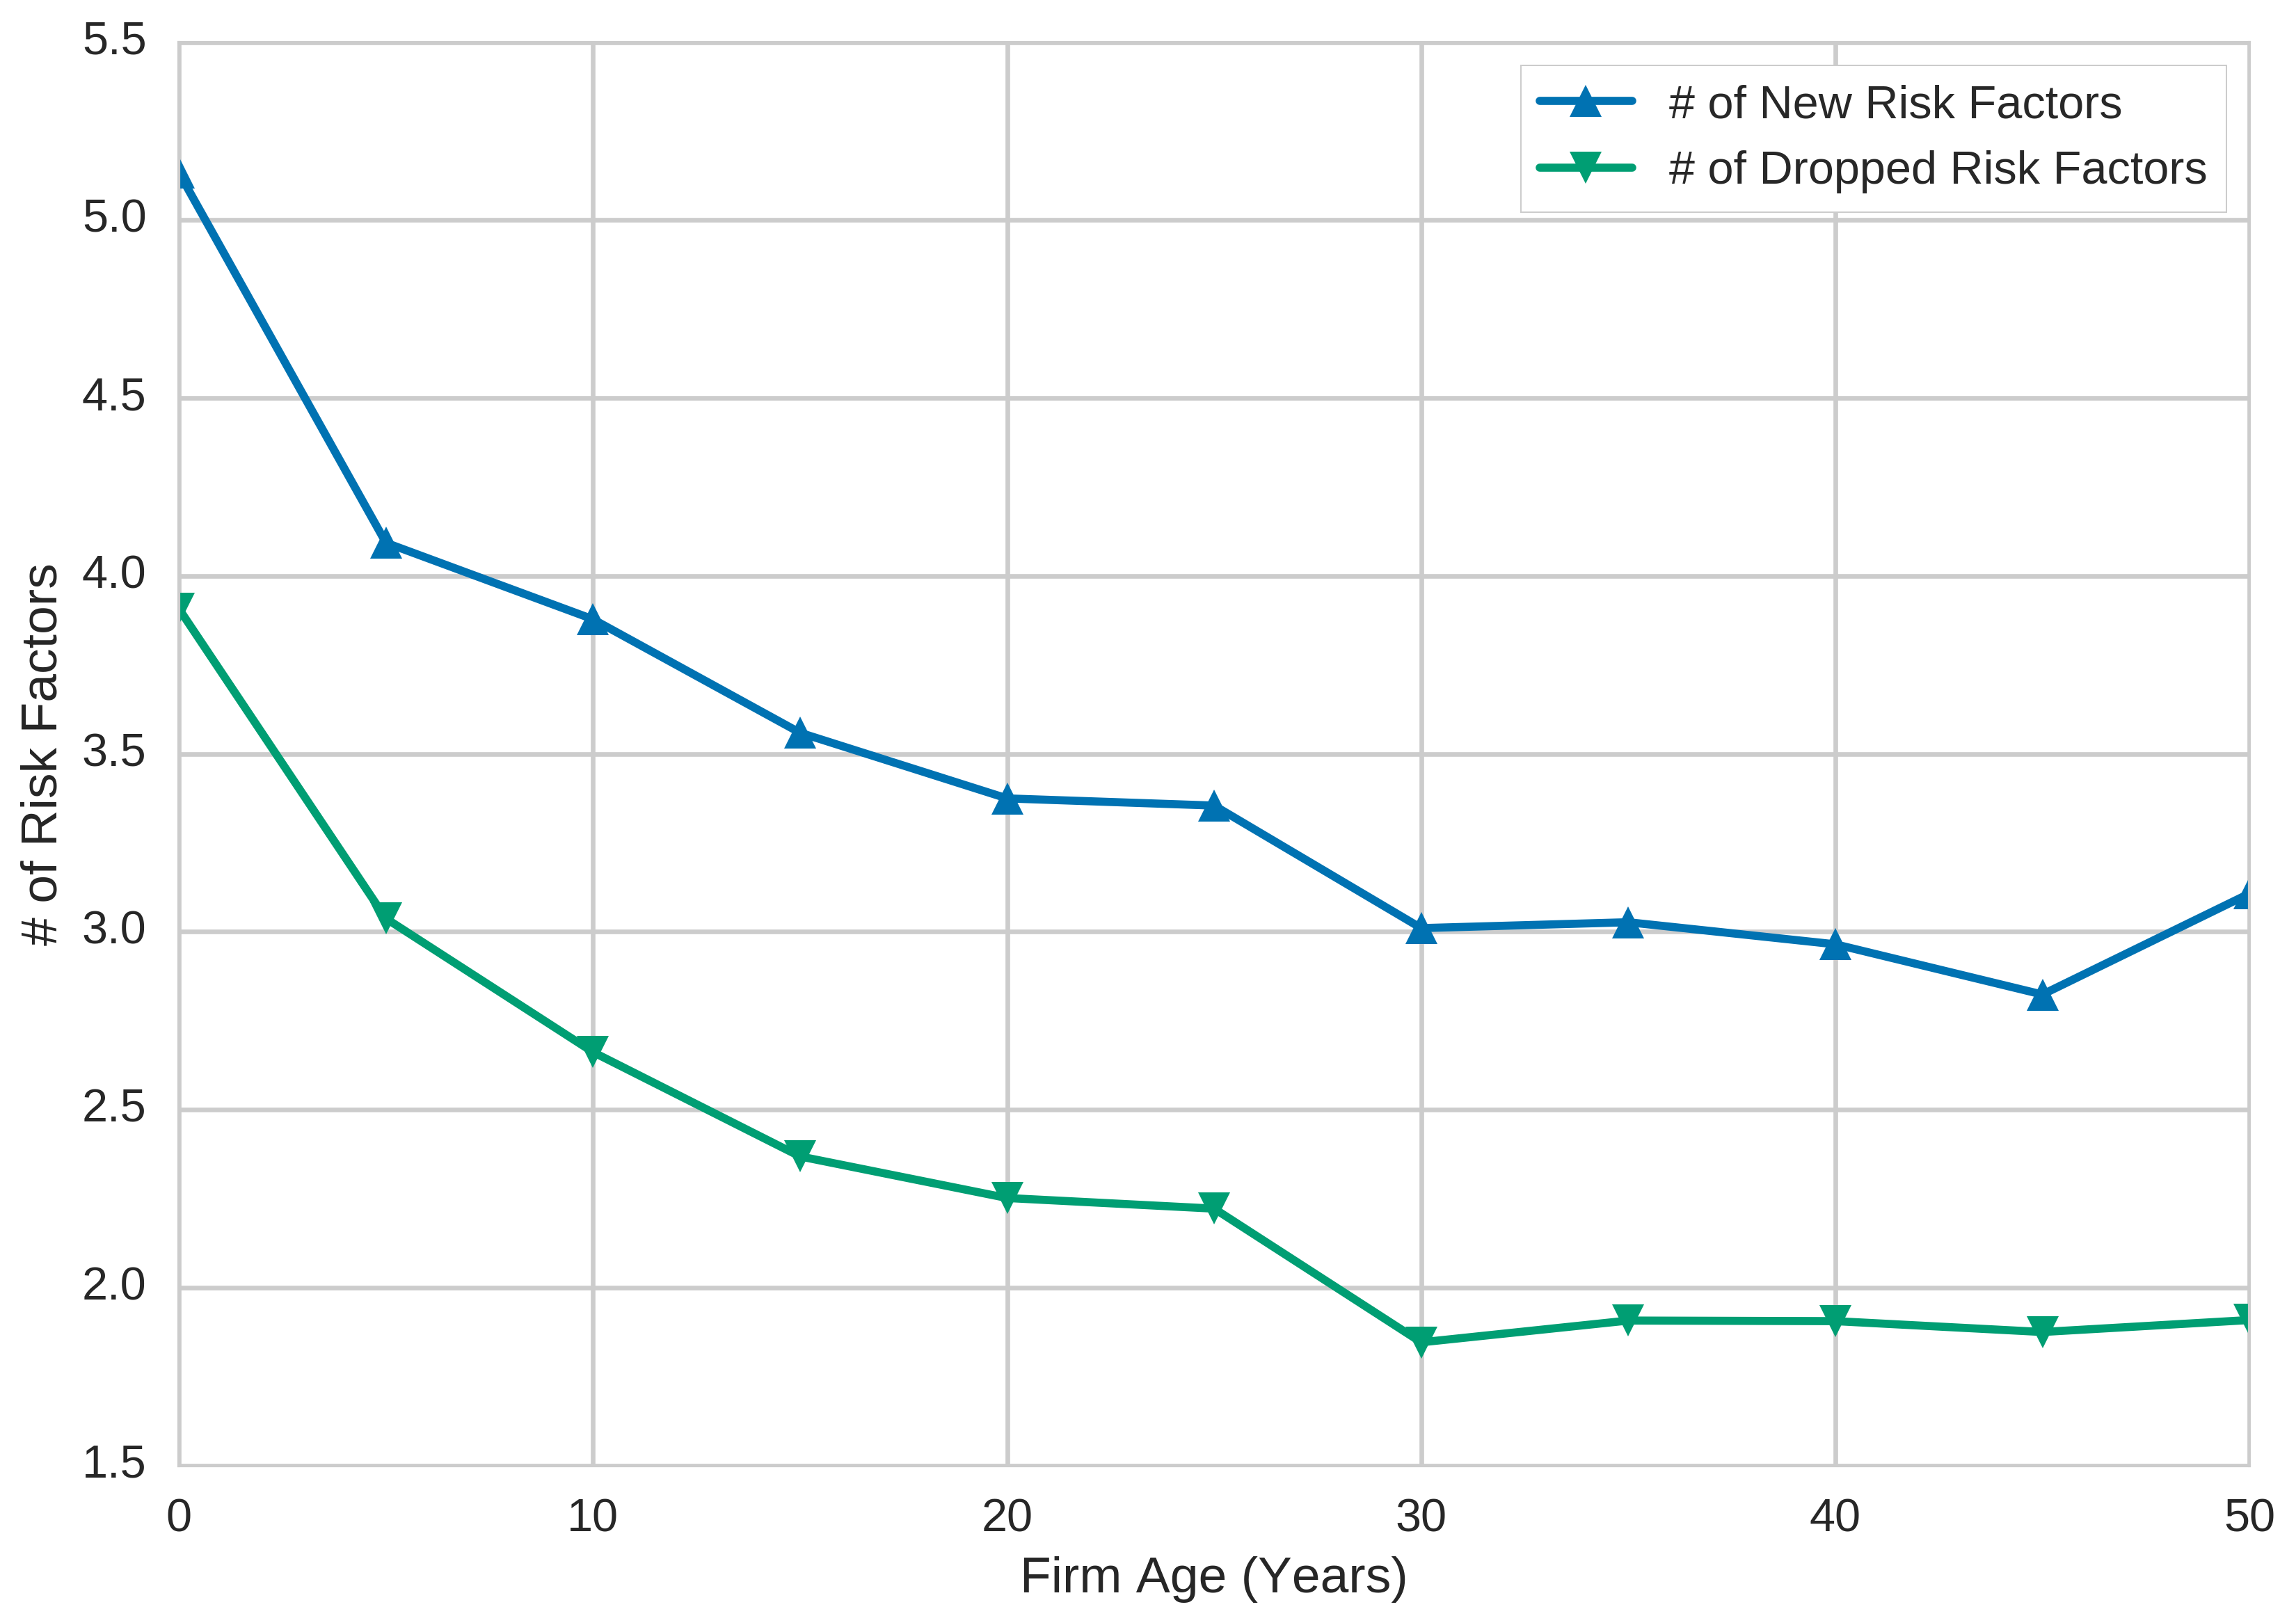
\includegraphics[scale=.5]{figures/add-drop_over_age.png}
\end{figure}




\section{Results}\label{sec:supply_result}

QED.




\subsection{Alternative Specifications}\label{sec:supply_robustness}

QED again.



\chapter{Conclusion} \label{ch:conclusion}
    %  .d8888b.                             888                   d8b
% d88P  Y88b                            888                   Y8P
% 888    888                            888
% 888         .d88b.  88888b.   .d8888b 888 888  888 .d8888b  888  .d88b.  88888b.
% 888        d88""88b 888 "88b d88P"    888 888  888 88K      888 d88""88b 888 "88b
% 888    888 888  888 888  888 888      888 888  888 "Y8888b. 888 888  888 888  888
% Y88b  d88P Y88..88P 888  888 Y88b.    888 Y88b 888      X88 888 Y88..88P 888  888
%  "Y8888P"   "Y88P"  888  888  "Y8888P 888  "Y88888  88888P' 888  "Y88P"  888  888

So say we all.


%%%%%%%%%%%%%%%%%%%%%%%%%%%%%%%%%%%%%%%%%%%%%%%%%%%%%%%%%%%%%%%%%%%%%%%%
%                            Bibliography                              %
%%%%%%%%%%%%%%%%%%%%%%%%%%%%%%%%%%%%%%%%%%%%%%%%%%%%%%%%%%%%%%%%%%%%%%%%
\clearpage
\phantomsection
\addcontentsline{toc}{chapter}{Bibliography}{} \label{ch:bibliography}
	{\singlespacing
		\bibliographystyle{./jf}
    % This is your *.bib file.
		\bibliography{./RFD}
	}


%%%%%%%%%%%%%%%%%%%%%%%%%%%%%%%%%%%%%%%%%%%%%%%%%%%%%%%%%%%%%%%%%%%%%%%%
%                             Appendices                               %
%%%%%%%%%%%%%%%%%%%%%%%%%%%%%%%%%%%%%%%%%%%%%%%%%%%%%%%%%%%%%%%%%%%%%%%%
\clearpage
\appendix
\phantomsection
\addcontentsline{toc}{chapter}{Appendices}

\chapter{Variable Descriptions} \label{App:vardef}
    { \bgroup
\singlespacing

The following table defines the variables used in this paper.
Variable names and calculations provided in brackets correspond to source database. For the regressions presented in the tables, the continuous variables are winsorized at the 1st and 99th percentiles.

\begin{center}
	\centering
	\def\arraystretch{1.25}
    \footnotesize
	\begin{longtable*}{l  >{\raggedright\let\newline\\\arraybackslash\hspace{0pt}}p{.7 \textwidth}}
        \toprule
		\textbf{Variable} 	& \textbf{Description} \\ \midrule 
		\endfirsthead
		\multicolumn{2}{c}{...continued from previous page.} \\
		\toprule
		\textbf{Variable} 	& \textbf{Description} \\ \midrule 
		\endhead
		\midrule
		\multicolumn{2}{c}{Continued on next page...} \\ 
		\endfoot
		\bottomrule
		\endlastfoot
		Assets				& Total assets $ \{ AT \} $  \\ %\hline
		Market Equity		& Market value of equity at fiscal year end. $ \{ CSHPRI * PRCC\_F \} $  \\ %\hline
		Net Income/AT 		& Net income to lagged assets. $ \{  NI_{t}/AT_{t-1}  \} $  \\ %\hline
		Operating Inc./AT 	& Operating income (after depreciation) to lagged assets. $ \{  OIADP_{t}/AT_{t-1}  \} $  \\ %\hline
		Sales Growth  		& Ratio of change in sales to lagged assets. $ \{  (SALE_t - SALE_{t-1})/AT_{t-1}  \} $  \\ %\hline
        Sales / AT  		& Sales to lagged assets. $ \{  SALE_t/AT_{t-1}  \} $  \\ %\hline
        Book Equity			& Book value of equity. $ \{ (TEQ_{t}|AT_{t} - LT_{t}) + TXDITC_{t} - PSTK_{t} \} $  \\ %\hline
		Book-to-Market  	& Book to market. $ \{ \text{Book Equity}_{t}/\text{Market Equity}_{t}  \} $  \\ %\hline
		Leverage  			& Leverage $ \{ (DLTT_{t} + DLC_{t})/AT_{t} \} $  \\ %\hline
		Tangibility  		& Tangibility $ \{ PPENT_{t}/AT_{t} \} $  \\ %\hline
		Turnover  			& Ratio of average daily volume (CRSP) to outstanding shares at fiscal year end (Compustat). \\ %\hline
		Beta  				& Market loading from CAPM model of daily returns on value weighted index, for all available days in the fiscal year. $ \{ RET = \alpha + \beta \cdot VWRETD + \epsilon \} $  \\ %\hline
        Excess Returns  	& Cumulative excess daily returns during fiscal year. $ \{ (\prod RET - VWRETD + 1) - 1  \} $  \\ %\hline
        Excess Ret. Std.	& Standard deviation of daily excess returns. $ \{ Std.\ Dev(RET- VWRETD)  \} $  \\ %\hline
        Min. Excess Ret.	& Minimum daily excess return during fiscal year. $ \{ Min(RET- VWRETD)  \} $  \\ %\hline
        Excess Ret. Skew	& Skewness of daily excess returns. $ \{ Skew(RET- VWRETD) \} $ \\ %\hline
        CAR$_{+3\ day}$  	& Cumulative abnormal return spanning three business days starting on the filing date of the annual report, using a Fama-French Carhart factor model. Data from Kenneth French's website. $ \{ RET=MKTRF+SMB+HML+UMD+MOM+\epsilon \}$ \\ %\hline
        CAR$_{+3\ months}$ 	& Cumulative abnormal return spanning 60 business days starting on the filing date of the annual report, using a Fama-French Carhart factor model. Data from Kenneth French's website. $ \{ RET=MKTRF+SMB+HML+UMD+MOM+\epsilon \}$ \\ %\hline
		Bid-Ask Spread$_{+1\ year}$ & Average daily bid ask spread at closing for 240 business days starting on the filing date of the annual report, as percentage of average bid and ask. $\{ 200*(ASK - BID)/(ASK + BID) \}$ \\ %\hline
		
		Negative NI 		& Indicator variable equal to 1 if next year's net income is negative. $ \{ NI_{t+1} < 0 \} $\\ %\hline
		Negative Op. Inc. 	& Indicator variable equal to 1 if next year's operating income is negative $ \{ OIADP_{t+1} < 0 \} $ \\ %\hline
		Sales Decline 		& Indicator variable equal to 1 if next year's sales are lower than the current year's sales by 10\%  or 10 million dollars, whichever is larger. $ \{ SALE_{t+1} - SALE_{t} < -10\%*max(100, SALE_{t}) \} $\\ %\hline
		Security Litigation	& Indicator variable equal to 1 if a securities litigation is filed in the subsequent year. \\ %\hline
		Lawsuit Intensity	& Natural log of number of litigation events found in CapitalIQ Key Developments database in a given fiscal year.\\ %\hline
		RF Comment 			& Indicator variable equal to 1 if an SEC comment letter is received in a given fiscal year that references risk factors. \\ %\hline
		Comment (Any) 		& Indicator variable equal to 1 if any SEC comment letter is received in a given fiscal year, including those with a reference to risk factors. \\ %\hline
		FPS Industry		& Indicator variable equal to 1 if the firm has an SIC code in one of the high litigation risk industries defined in \cite{francis_1994}. \\ %\hline
        
		\# Risk Factors 	& Total number of risk factors disclosed under Item 1A of an annual report. \\ %\hline
		\# New RF 			& Number of new risk factors which were not present in the previous year's annual report. \\ %\hline
   		\# Dropped RF 		& Number of risk factors which were in the previous year's annual report, but are no longer included in the present year.\\ %\hline
		\# Kept RF 			& Number of risk factors which were in the previous year's annual report and persist in the current annual report.\\ %\hline
		\# of Words 		& Total number of words in Item 1A of an annual report (excluding stop words). \\ %\hline
		\# of Sentences 	& Total number of sentences in Item 1A of an annual report.\\ %\hline
		\# of Specific Words& Total number of words identified by the Stanford Named Entity Recognition algorithm as being in categories: Location, Person, Organization \\ %\hline
		\# of Numerics 		& Total number of numbers in Item 1A of an annual report. \\ %\hline
		\# of Words/RF 		& Ratio of the total number of words to the total number of risk factors in Item 1A of an annual report (excluding stop words).\\ %\hline
		Specificity 		& Ratio of the total number of specific words to the total number of risk factors in Item 1A of an annual report (excluding stop words).\\ %\hline
		Numeric Intensity 	& Ratio of the total number of numbers to the total number of risk factors in Item 1A of an annual report (excluding stop words).\\ %\hline
		FOG Index 			& Gunning Fog score for the text in Item 1A of an annual report (excluding stop words). Calculated as $\left\{ 0.4 \left(\frac{\# \ of\ words}{\#\ of\ sentences} + 100\frac{\#\ of\ complex\ words}{\#\ of\ words}\right) \right\}$ \\ %\hline
		
	\end{longtable*}
\end{center}
\egroup
}

\chapter{Risk Factor Extraction} \label{App:scraping}
    \noindent

To derive an initial list of filings, I extract the gvkey and historical CIKs from the Compustat annual file, starting from 89,687 firm years.
I then merge the non-missing CIKs from Compustat with the EDGAR filings index file provided by the SEC.%
  \footnote{Located, for example, at
            \bluehref{ftp://ftp.sec.gov/edgar/full-index/2005/QTR1/}{ftp.sec.gov/edgar/full-index/2005/QTR1/master.idx}.
            Downloaded using script from
            \bluehref{https://github.com/gaulinmp/pyedgar/blob/master/pyedgar/downloader.py}{github.com/gaulinmp/pyedgar}}
I filter the index files to include only form 10-Ks, excluding amended 10-K/As, leaving 67,648 filings from 9,632 firms.
Form 10-KSB is also included, but are no longer filed after 2009.

\end{document}
